\documentclass{article}
\usepackage[utf8]{inputenc}
\usepackage{geometry}
\geometry{a4paper, top=30mm, bottom=25mm, left=20mm, right=20mm}
\usepackage{tzplot}
\usepackage{amsmath}
\usepackage[utopia]{mathdesign}
\usepackage{kinematikz}
\usepackage{tasks}
\newcommand{\ans}{\textcolor{red!95}{\textit{\quad Ans.}}}
\title{Module-Test-7\\(Physics-NEET)}
%\newcommand{\ansit}{\textcolor{red!95}{\textit{\quad }}}
\def\ansit#1{\textcolor{red!95}{\quad}}

%\usepackage[italicdiff]{physics}
\usepackage{physunits}
\tikzstyle test-paper=[>=latex, thick]
\tikzset{
>=latex
}
\tikzstyle{block}=[rectangle,draw, thick, minimum size=8mm, node distance=1.8cm,]
\tikzstyle{pulley}=[circle,draw, thick, minimum size=10mm, node distance=1.8cm]

\tikzstyle{sblock}=[rectangle,draw, thick, minimum size=8mm, node distance=1.8cm]
\tikzstyle{spulley}=[circle,draw, thick, minimum size=8mm, node distance=1.8cm]

\tikzstyle{lblock}=[rectangle,draw, thick, minimum size=12mm, node distance=1.8cm]
\tikzstyle{lpulley}=[circle,draw, thick, minimum size=12mm, node distance=2cm]

\tikzstyle{hblock}=[rectangle,draw, thick, minimum height=12mm, minimum width=20mm, node distance=1.8cm]
\tikzstyle{Hblock}=[rectangle,draw, thick, minimum height=12mm, minimum width=24mm, node distance=1.8cm]
\tikzstyle{lift}=[rectangle,draw, thick, minimum height=60mm, minimum width=50mm, node distance=1.8cm]

\tikzstyle{Bpulley}=[circle,draw, thick, minimum size=20mm, node distance=1.8cm]

\tikzstyle{plank}=[rectangle,draw, thick, minimum height=8mm, minimum width=50mm, node distance=1.8cm]



% 1. Laws of motion (1 to 22)
% 2. Projectile Motion (23 to 24)
% 3. Kinematics (25 to 27)
% 4. Work-Energy (28-30)

\begin{document}
\maketitle


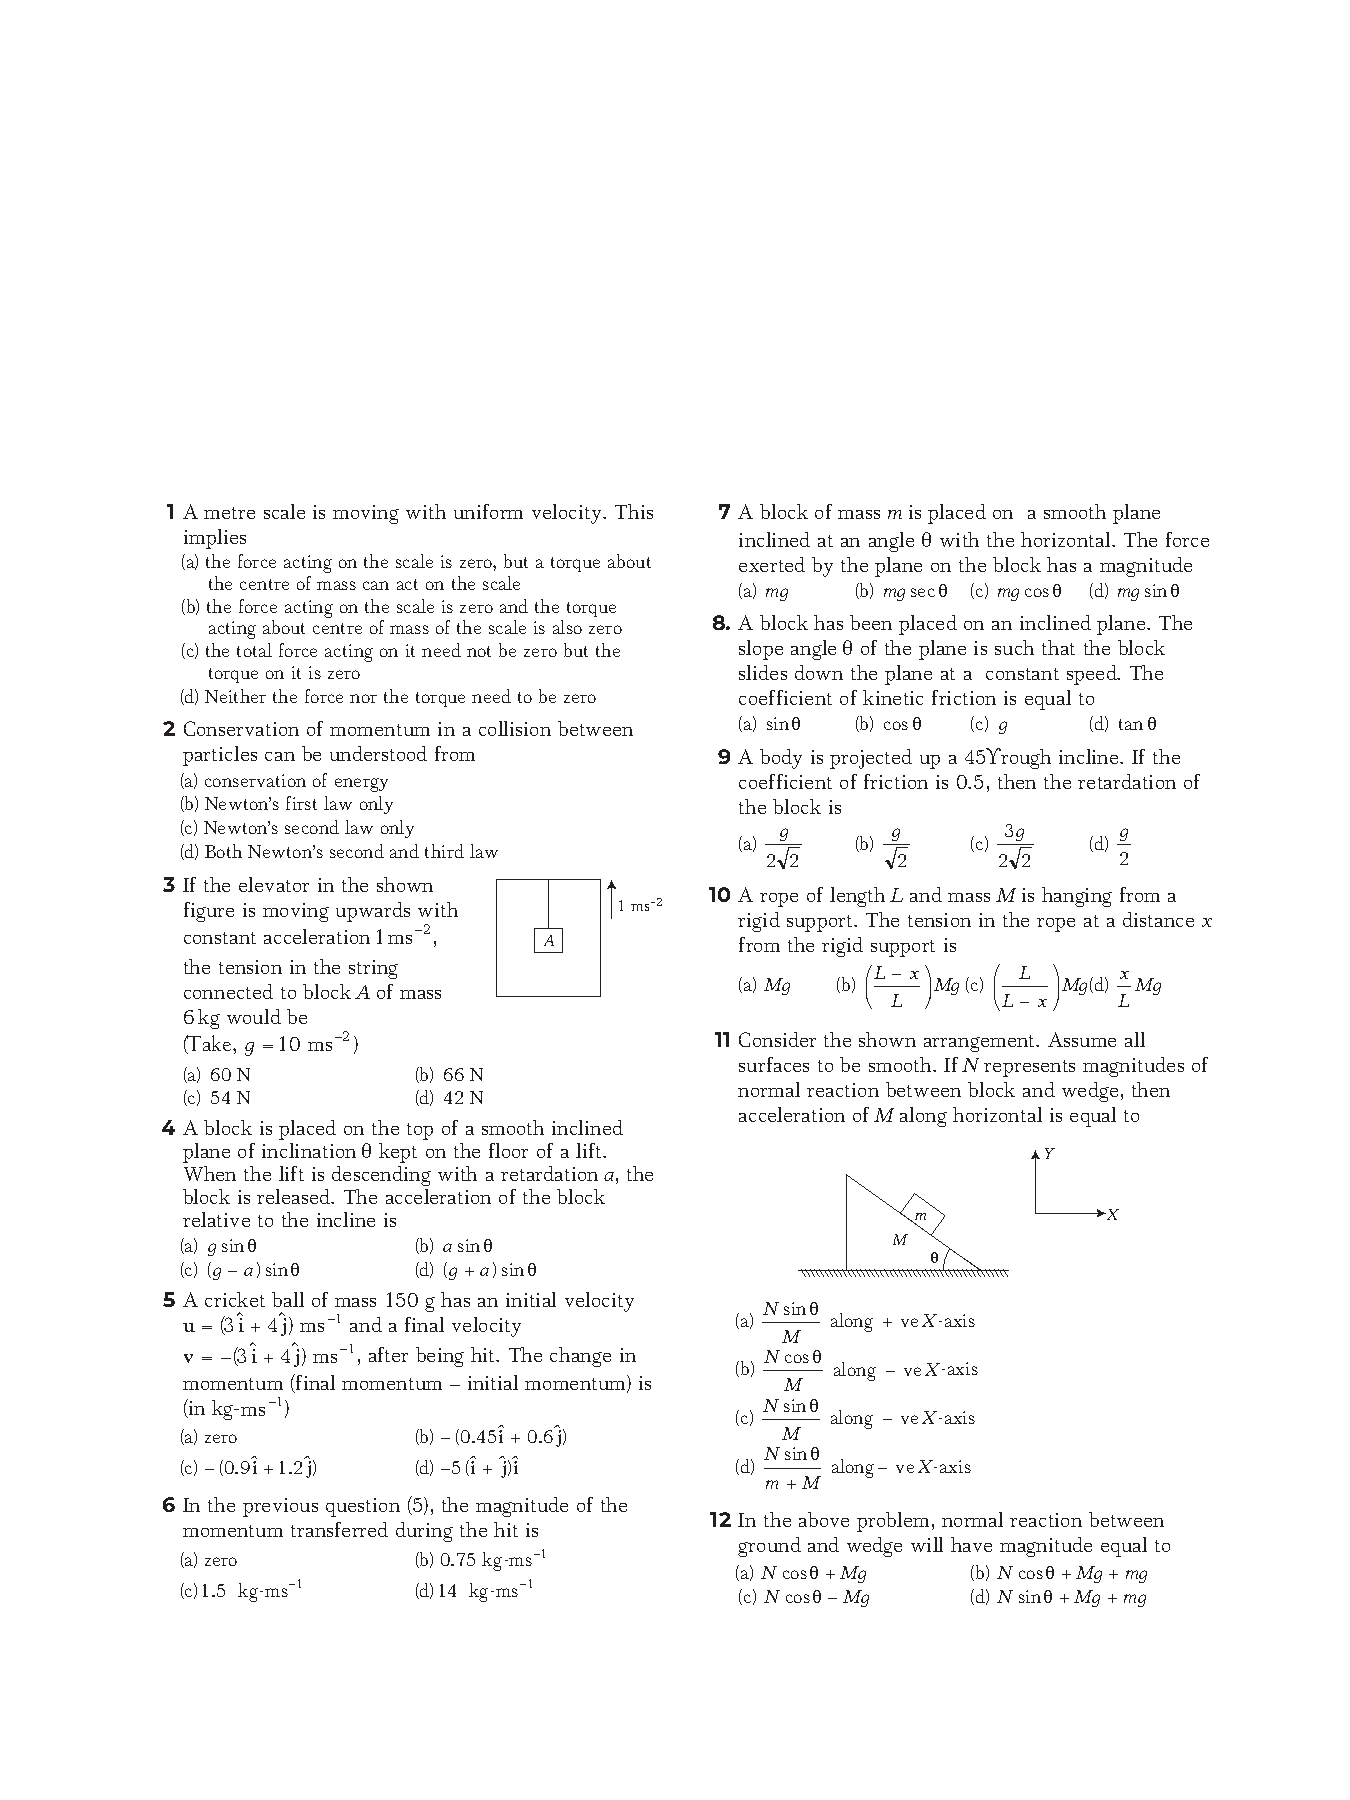
\includegraphics[trim={2.5cm 0 2cm 0},clip, width=170 mm]{p1-12}
\linebreak
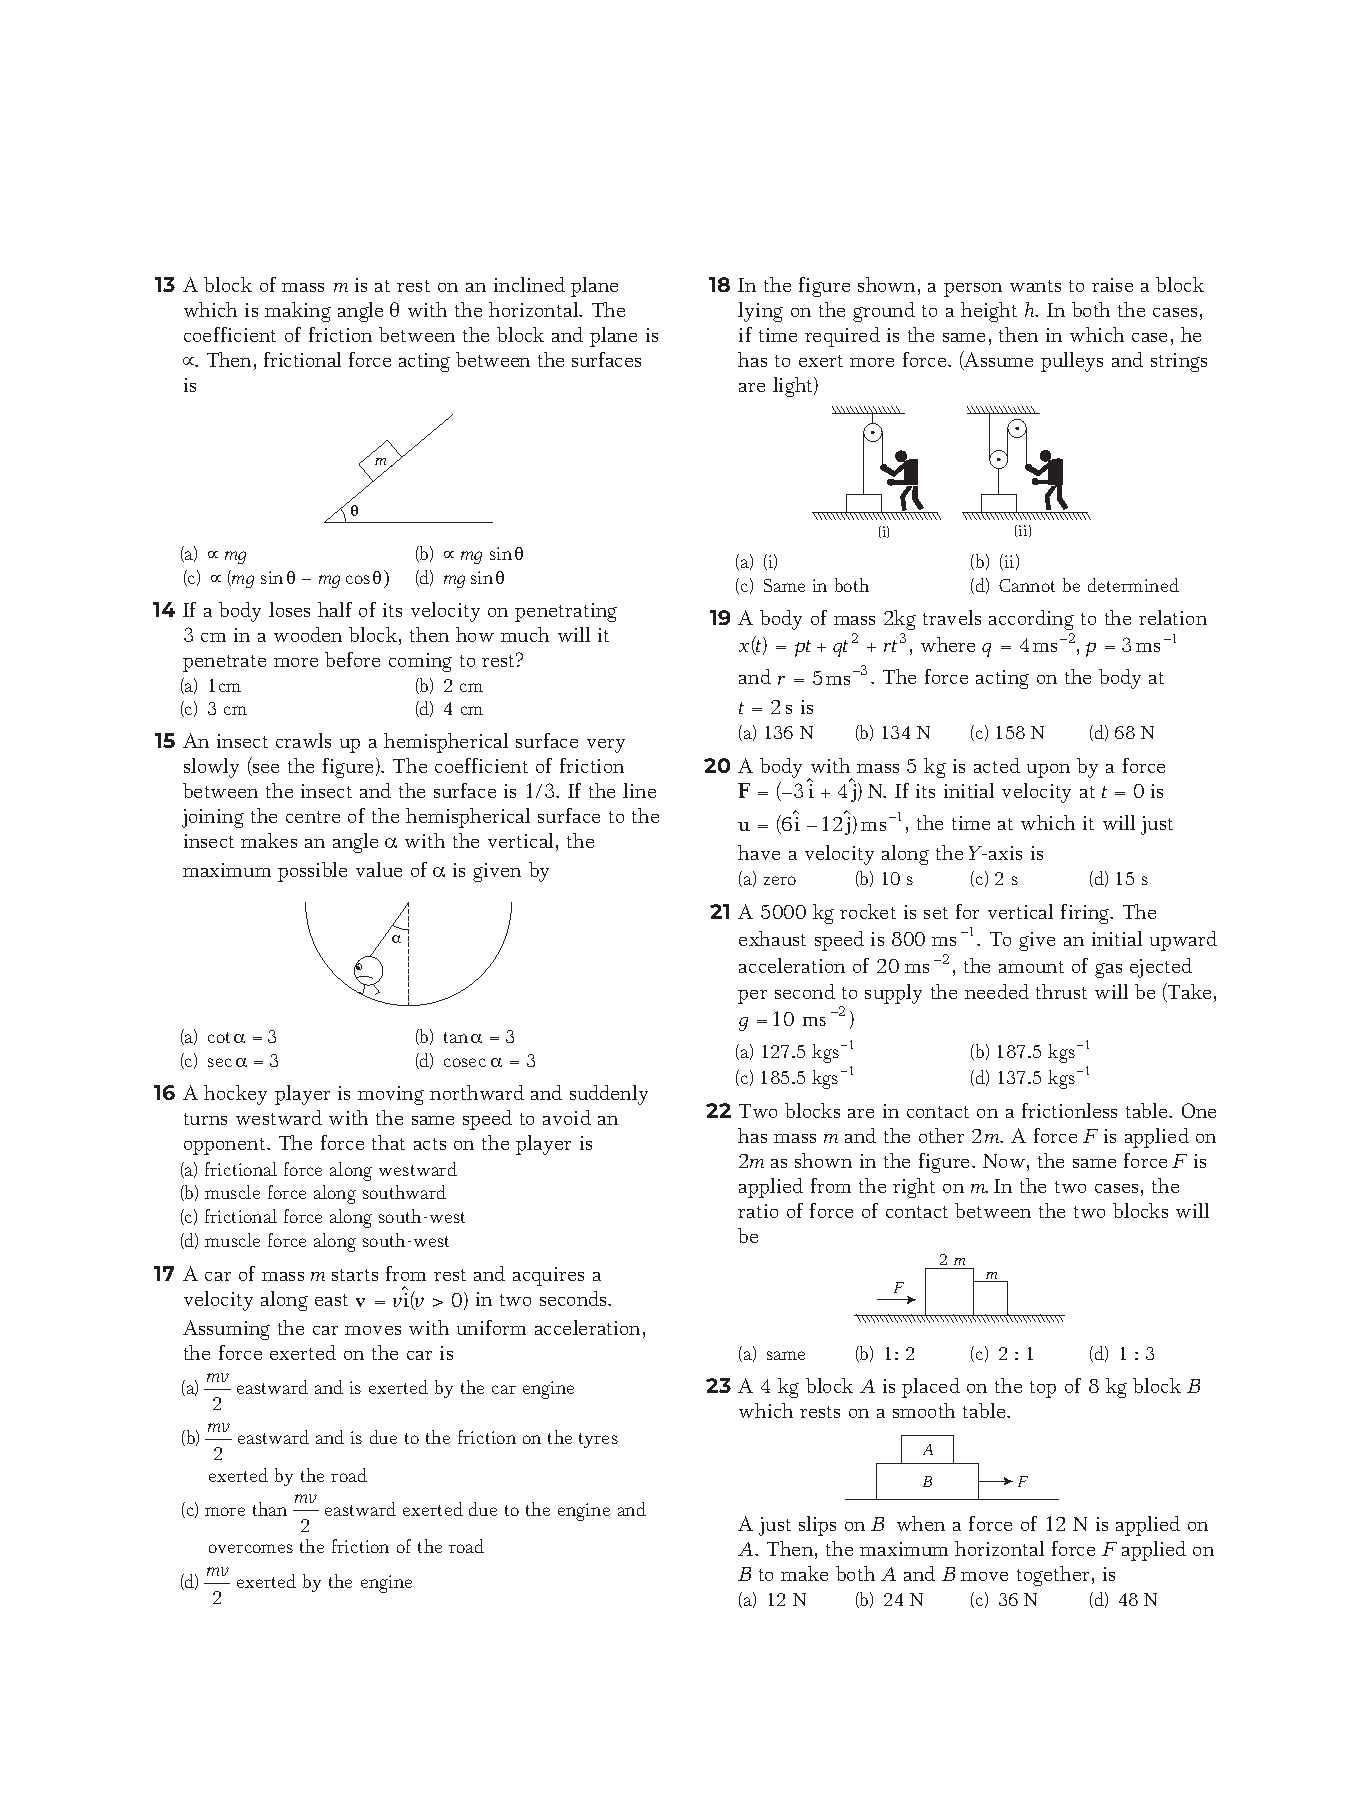
\includegraphics[trim={2.5cm 0 2cm 0},clip, width=170 mm]{p13-23}
\linebreak
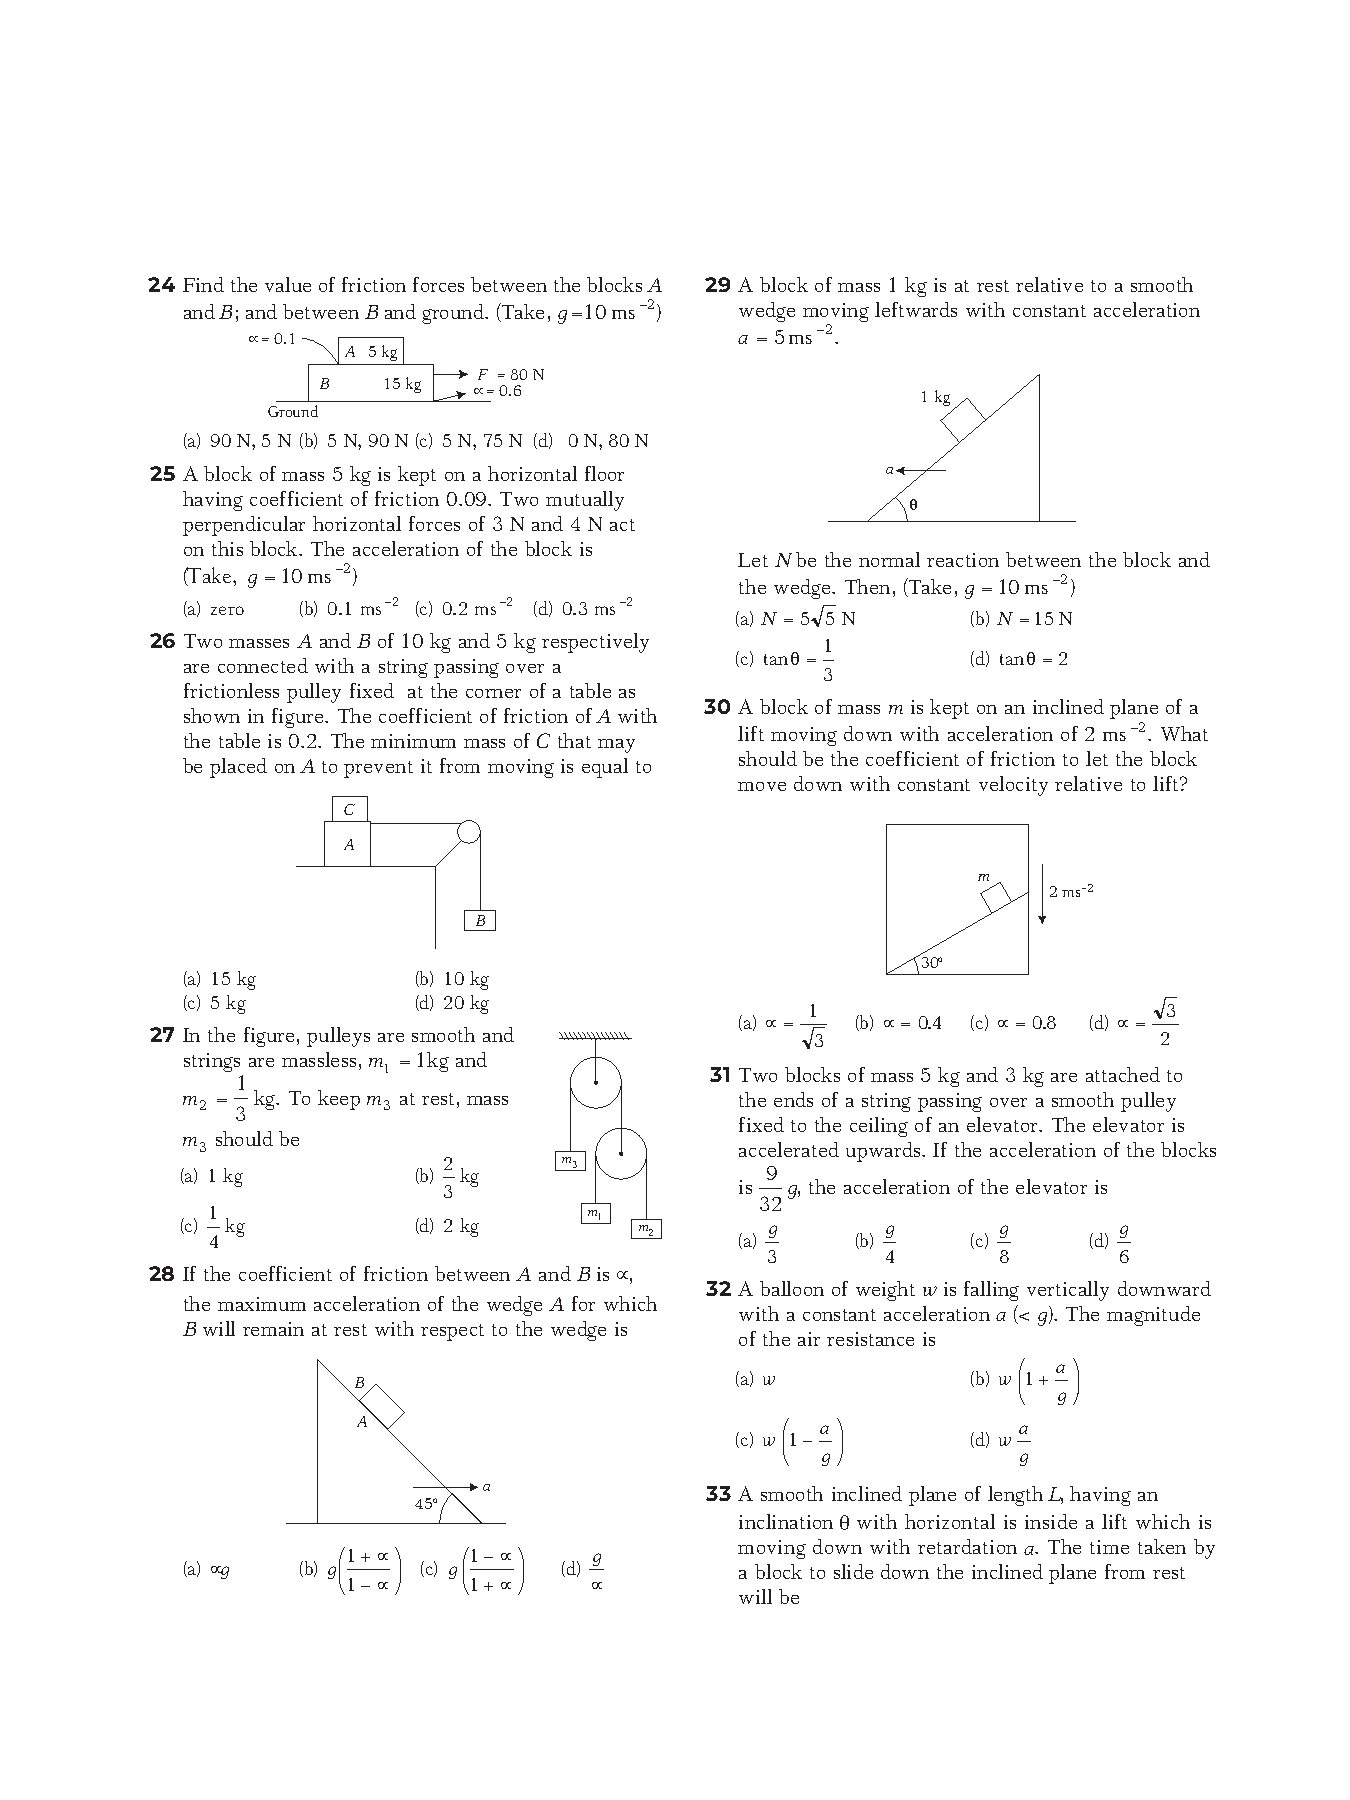
\includegraphics[trim={2.5cm 0 2cm 0},clip, width=170 mm]{p24-33}
\linebreak
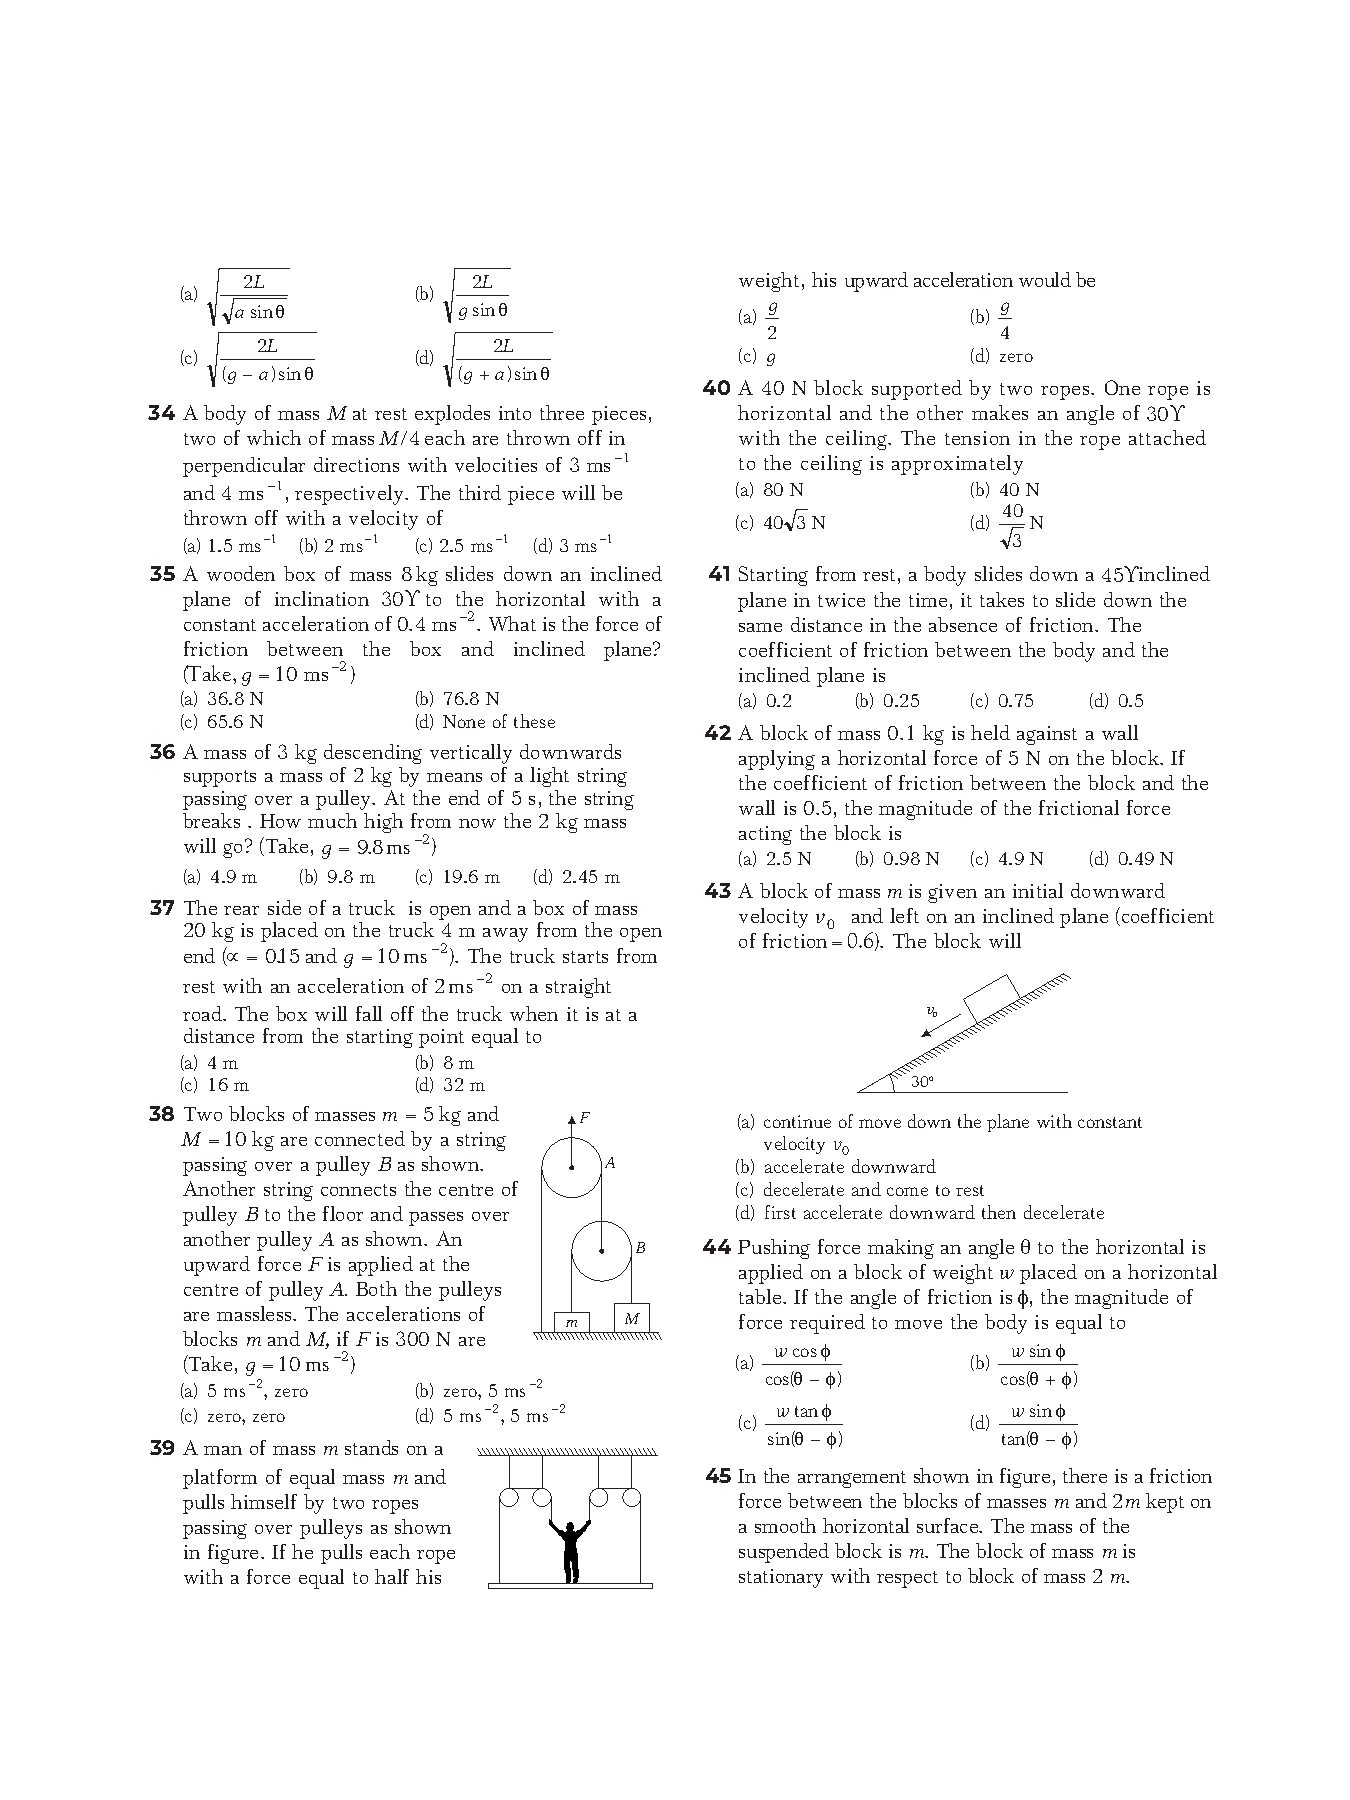
\includegraphics[trim={2.5cm 0 2cm 0},clip, width=170 mm]{p34-45}
\linebreak
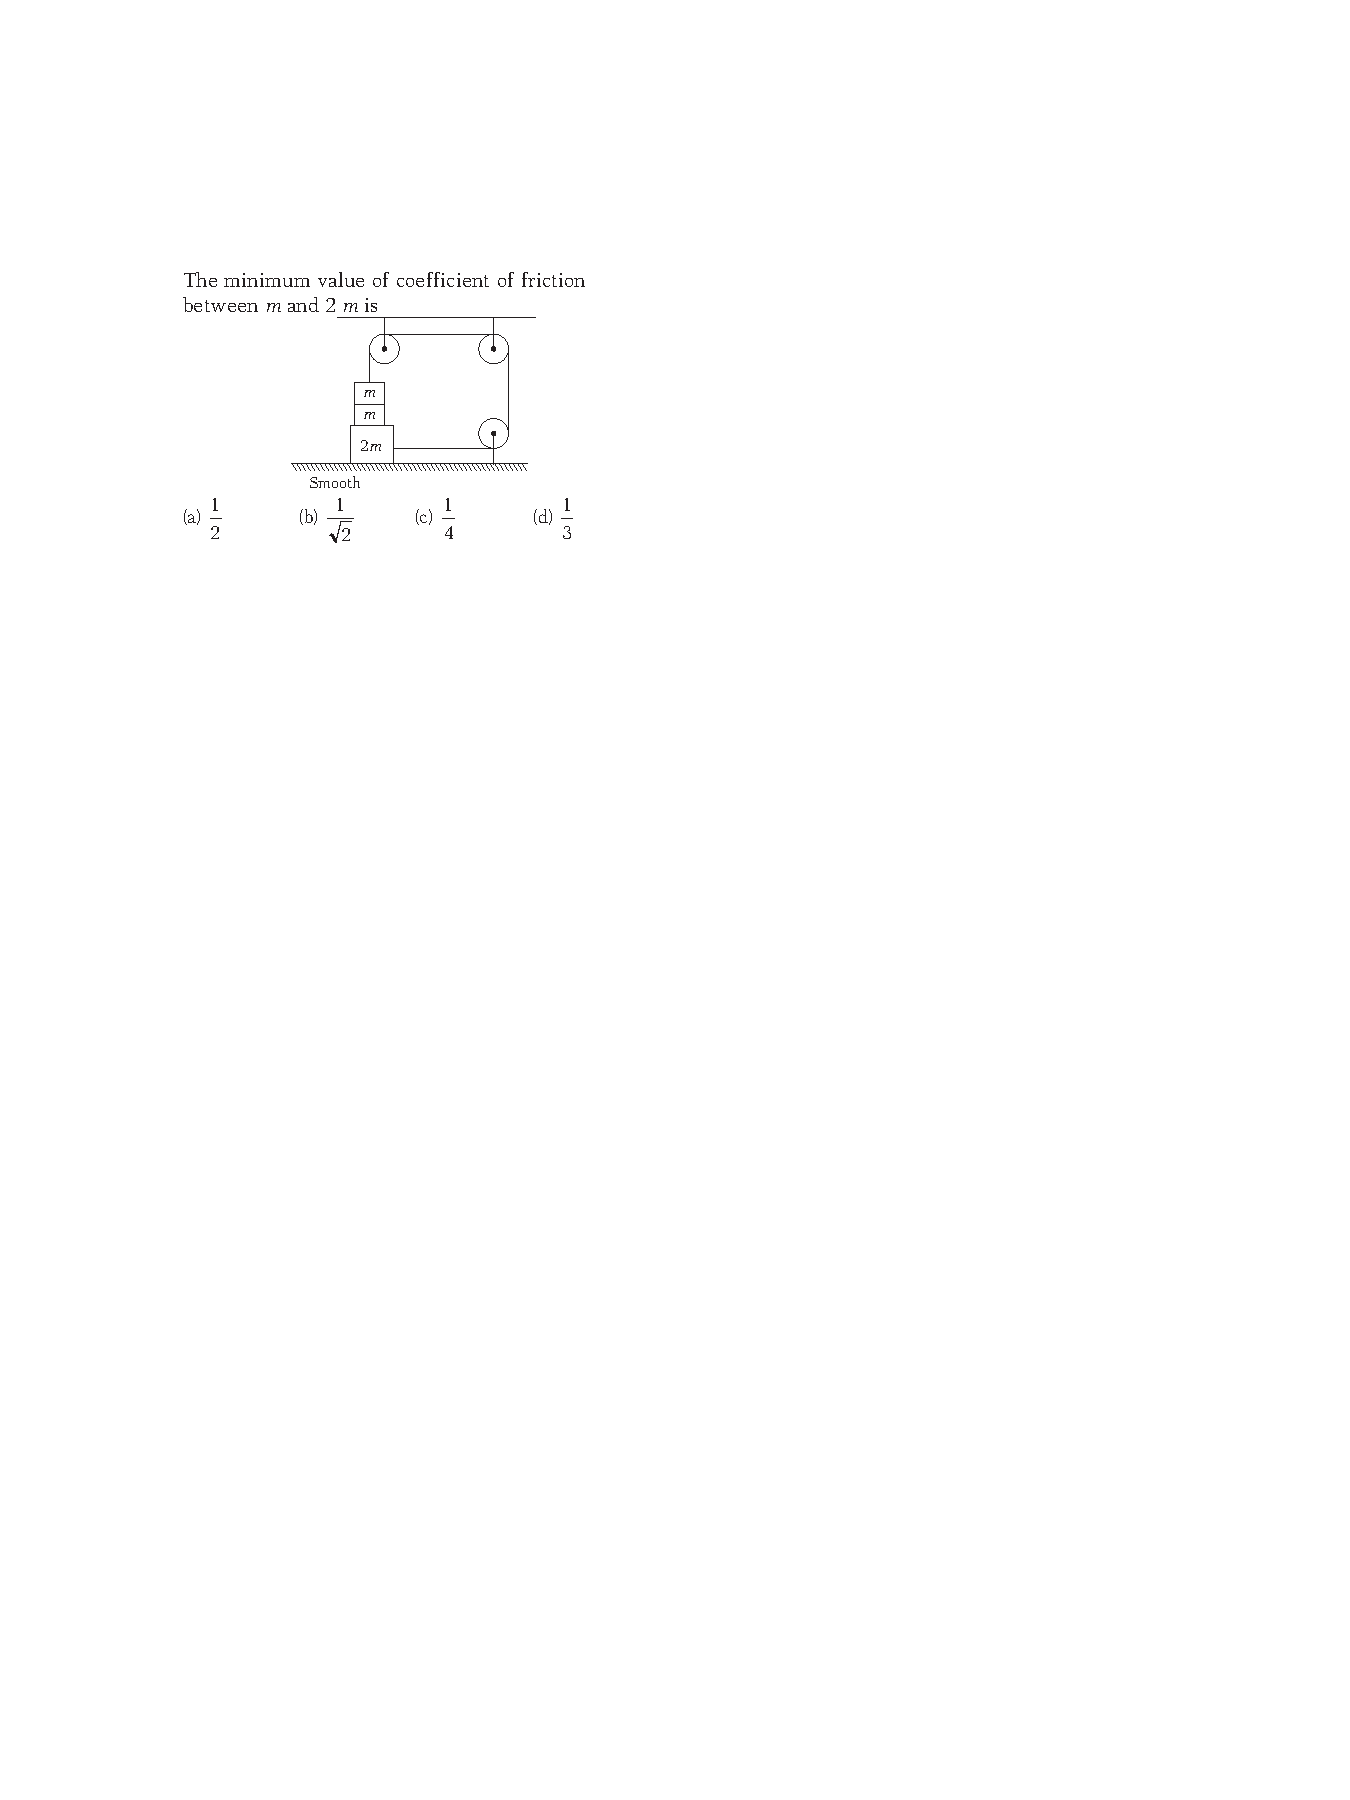
\includegraphics[trim={2.5cm 0 0.5cm 0},clip, width=80 mm]{p45}


\hrule

\pagebreak

\begin{center}
\texttt{A.N.S.W.E.R.}
\end{center}


\begin{tasks}[label=\arabic*.](2)
	\task (b)
	\task (d)
	\task (b)
	\task (c)
	\task (c)
	\task (c)
	\task (c)
	\task (d)
	\task (c)
	\task (b)
	\task (c)
	\task (a)
	\task (d)
	\task (a)
	\task (a)
	\task (d)
	\task (b)
	\task (a)
	\task (a)
	\task (b)
	\task (b)
	\task (b)
	\task (b)
	\task (d)
	\task (b)
	\task (a)
	\task (a)
	\task (b)
	\task (a)
	\task (a)
	\task (c)
	\task (c)
	\task (d)
	\task (c)
	\task (a)
	\task (a)
	\task (a)
	\task (a)
	\task (d)
	\task (a)
	\task (c)
	\task (b)
	\task (c)
	\task (b)
	\task (c)
\end{tasks}
\hrule





\end{document}
